\documentclass{article}
\title{Tarea final del Módulo 3 "Principios psicométricos en las evaluaciones"}
\author{Salvador Enrique Rodríguez Hernández}
\date{\today} % para que no aparezca la fecha la dejo en blanco

\usepackage{Sweave}
\begin{document}
\Sconcordance{concordance:Documento_de_prueba.tex:Documento_de_prueba.Rnw:%
1 2 1 1 0 4 1 1 52 1 2 22 0 1 2 1 3 18 0 1 2 1 0 1 3 2 1 1 2 18 0 1 2 1 %
0 1 2 4 1 1 3 1 2 74 1}


\maketitle

\textbf{I. Análisis inicial}\\ 
1. Omisiones


A partir de la tabla de frecuencias anterior, se concluye que no hay omisiones. 

\begin{Schunk}
\begin{Sinput}
> distribucion_respuestas
\end{Sinput}
\begin{Soutput}
        Correcto Incorrecto No_responde
ítem 1      6264        660           0
ítem 2      5339       1585           0
ítem 3      3578       3346           0
ítem 4      5138       1786           0
ítem 5      1944       4980           0
ítem 6      2342       4582           0
ítem 7      4425       2499           0
ítem 8      3936       2988           0
ítem 9      5553       1371           0
ítem 10     3526       3398           0
ítem 11     3249       3675           0
ítem 12     4644       2280           0
ítem 13     3517       3407           0
ítem 14      739       6185           0
ítem 15     2564       4360           0
\end{Soutput}
\end{Schunk}

2.	ítems en los que se observa una alta proporción de respuestas (mayor de 0.5). 

\begin{Schunk}
\begin{Soutput}
         Correcto Incorrecto No_responde
ítem 1  0.9046794 0.09532062           0
ítem 2  0.7710861 0.22891392           0
ítem 3  0.5167533 0.48324668           0
ítem 4  0.7420566 0.25794339           0
ítem 5  0.2807626 0.71923744           0
ítem 6  0.3382438 0.66175621           0
ítem 7  0.6390815 0.36091854           0
ítem 8  0.5684575 0.43154246           0
ítem 9  0.8019931 0.19800693           0
ítem 10 0.5092432 0.49075679           0
ítem 11 0.4692374 0.53076256           0
ítem 12 0.6707106 0.32928943           0
ítem 13 0.5079434 0.49205661           0
ítem 14 0.1067302 0.89326979           0
ítem 15 0.3703062 0.62969382           0
\end{Soutput}
\end{Schunk}
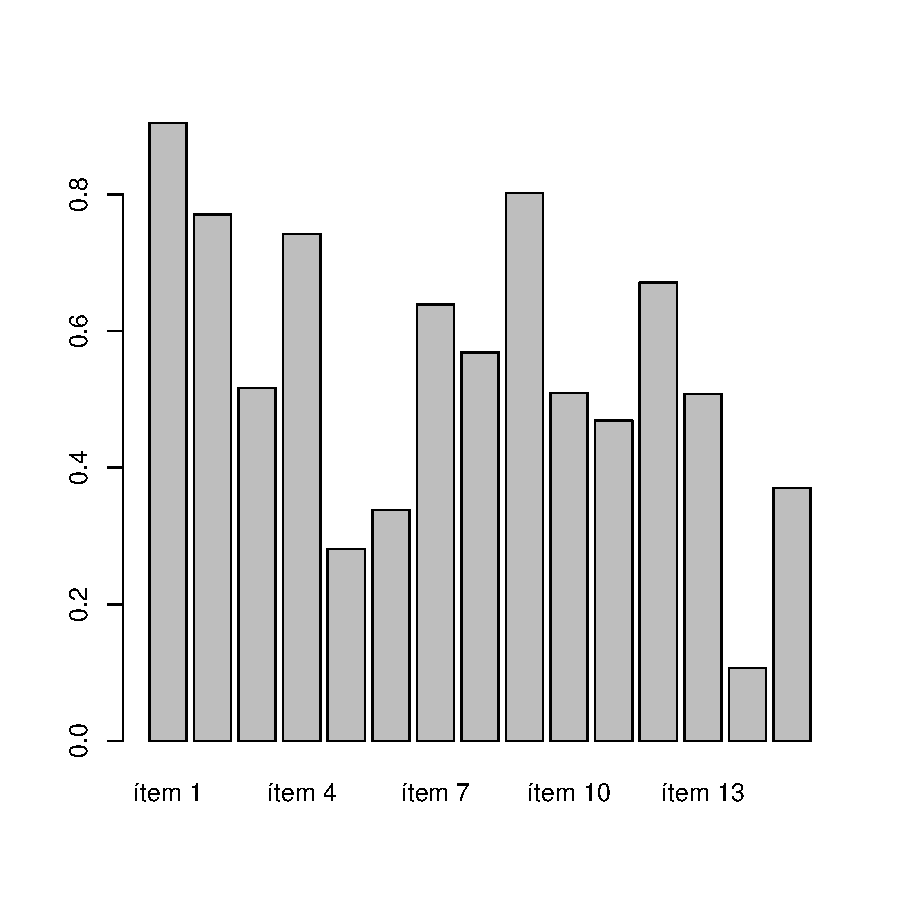
\includegraphics{Documento_de_prueba-003}

A partir de la tabla y gráfica anterior, se observa que los ítems con una proporción de respuestas correctas mayor a 0.5, son los ítems 1, 2, 3, 4, 7, 8, 9, 10, 12, 13. \\ 

3.	ítems con alto porcentaje de respuestas incorrectas (mayor del 50) 

\begin{Schunk}
\begin{Soutput}
        Correcto Incorrecto No_responde
ítem 1  90.46794   9.532062           0
ítem 2  77.10861  22.891392           0
ítem 3  51.67533  48.324668           0
ítem 4  74.20566  25.794339           0
ítem 5  28.07626  71.923744           0
ítem 6  33.82438  66.175621           0
ítem 7  63.90815  36.091854           0
ítem 8  56.84575  43.154246           0
ítem 9  80.19931  19.800693           0
ítem 10 50.92432  49.075679           0
ítem 11 46.92374  53.076256           0
ítem 12 67.07106  32.928943           0
ítem 13 50.79434  49.205661           0
ítem 14 10.67302  89.326979           0
ítem 15 37.03062  62.969382           0
\end{Soutput}
\end{Schunk}
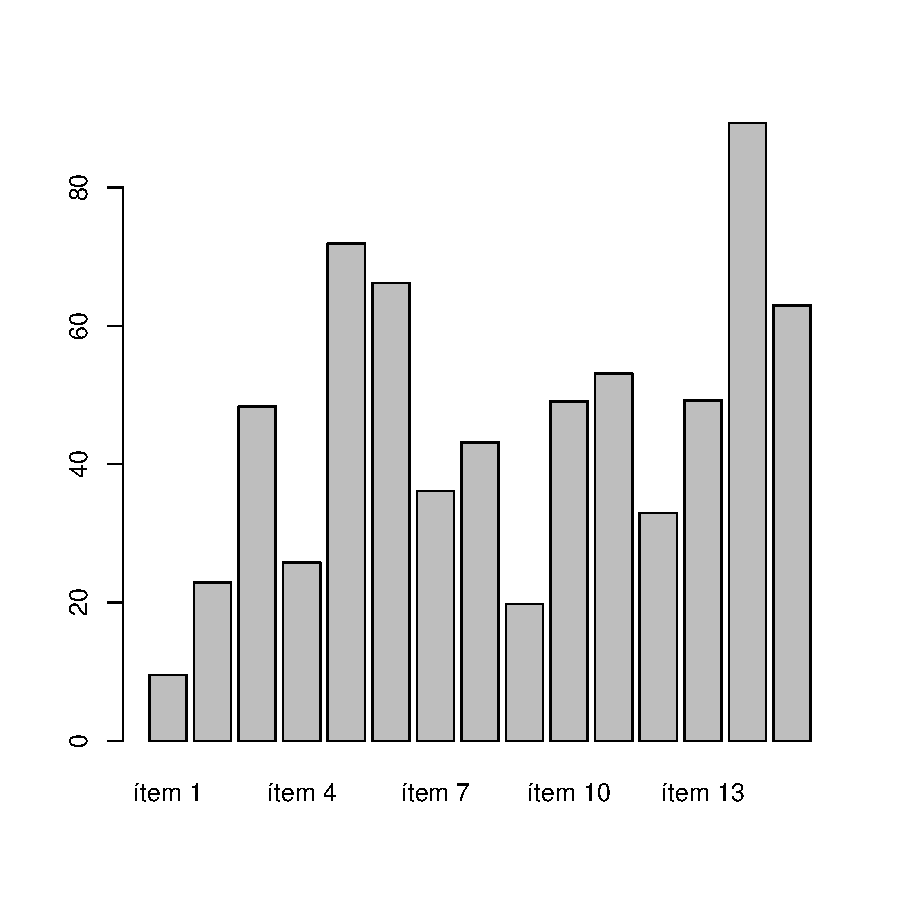
\includegraphics{Documento_de_prueba-004}

A partir de la tabla y gráfica anterior, se observa que los ítems con un porcentaje de respuestas incorrectas mayor al 50 por ciento, son los ítems 5, 6, 11, 14, 15.\\

\textbf{II.	Análisis Global del Test}\\
1. Histograma de los resultados totales

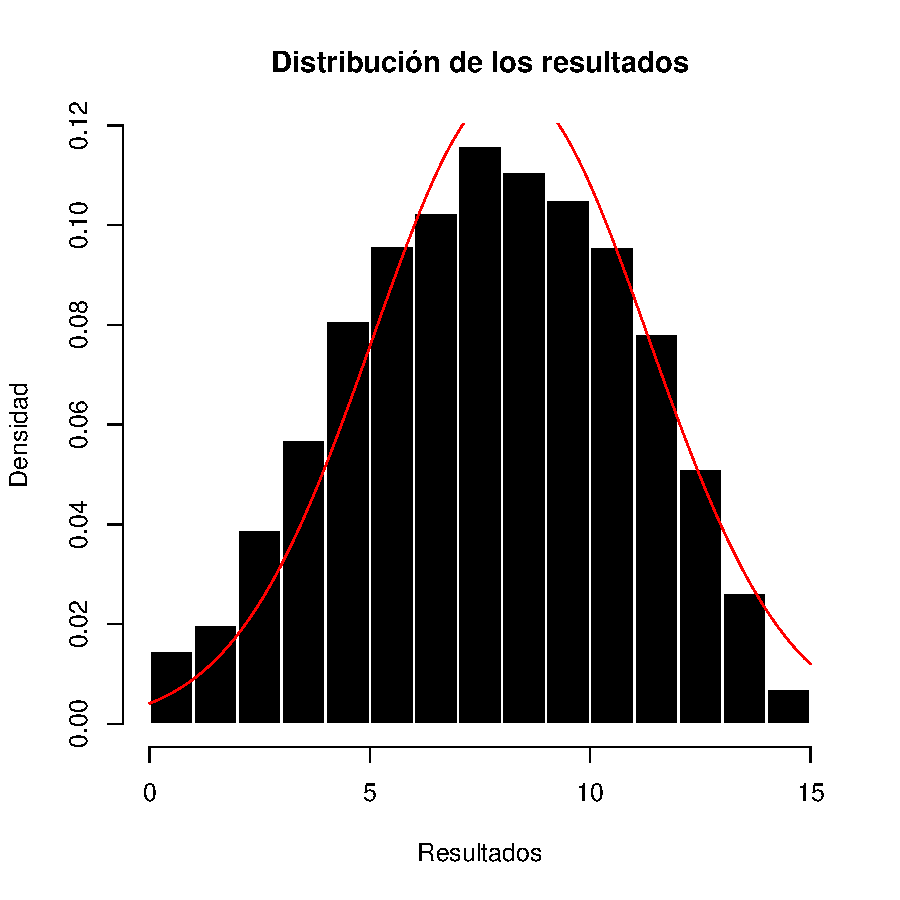
\includegraphics{Documento_de_prueba-005}

2. Estadísticos

\begin{center}
 \begin{tabular}{||c c||} 
 \hline
 Estadístico & Valor \\ [0.5ex] 
 \hline\hline
 Puntaje Mínimo & 0  \\ 
 \hline
 Puntaje Máximo & 15  \\
 \hline
 Media Aritmética & 8.2  \\
 \hline
 Desviación Estándar & 3.12 \\
 \hline
 Coeficiente de Asimetría & -0.14 \\ [1ex] 
 \hline
\end{tabular}
\end{center}

3. Por el hecho de que el valor de la desviación estándar no es alto se podría considerar que el valor de la media es un buen estadístico de tendencia central de los datos. \\

4. De entrada informa que la distribución tiene una asimetría negativa, pero no tan marcada por el hecho que el valor no está tan alejado de 0. \\

5. , All ver el histograma de la distribución, se puede apreciar que es una distribución que se asemaja a la normal, por lo que era esperable que el valor de la media fuera representativo de la distribución de los datos, al mismo tiempo se esperaría que el coeficiente de asimetría no tuviera un valor tan alto, siendo cercano a cero, refiriendo así a una distribución simétrica.\\ 
\textbf{III. Análisis individual de los ítems.} \\
1. Grado de dificultad de cada ítem 

\begin{center}
 \begin{tabular}{||c c||} 
 \hline
 ítem & Grado de dificultad (valor) \\ [0.5ex] 
 \hline\hline
 1 &   0.90 \\ 
 \hline
 2 & 0.77  \\
 \hline
 3 & 0.52  \\
 \hline
 4 & 0.74 \\
 \hline
  5 & 0.28 \\
 \hline
  6 & 0.34 \\
 \hline
  7 & 0.64 \\
 \hline
  8 & 0.57 \\
 \hline
  9 & 0.80 \\
 \hline
  10 & 0.51 \\
 \hline
  11 & 0.47 \\
 \hline
  12 & 0.67 \\
 \hline
  13 & 0.51 \\
 \hline
  14 & 0.11 \\
 \hline
  15 & 0.37 \\
 \hline
\end{tabular}
\end{center}

3. Correlación ítem - rest

\begin{Schunk}
\begin{Soutput}
   Variable Item.Total Alpha.Without    N
1        i1  0.2134460     0.7320506 6924
2        i2  0.3883730     0.7166717 6924
3        i3  0.2623227     0.7302432 6924
4        i4  0.2765054     0.7275937 6924
5        i5  0.2860795     0.7267641 6924
6        i6  0.3857612     0.7162459 6924
7        i7  0.3494416     0.7202431 6924
8        i8  0.3702134     0.7179206 6924
9        i9  0.2762727     0.7273339 6924
10      i10  0.3335788     0.7221570 6924
11      i11  0.4250689     0.7115084 6924
12      i12  0.4332876     0.7110279 6924
13      i13  0.4213264     0.7119401 6924
14      i14  0.1957348     0.7332713 6924
15      i15  0.3835731     0.7164276 6924
\end{Soutput}
\end{Schunk}

4. Según las correlaciones mostrada en la tabla anterior, se tiene que los ítems 1, 3, 4, 9 y 14, deberían  ser excluidos por el hecho que su correlación con el resto de los ítems es menor que 25.\\
El hacer nuevamente el cálculo de las correlaciones, excluyendo los ítems antes mencionados, se tiene la siguiente tabla:

\begin{Schunk}
\begin{Soutput}
   Variable Item.Total Alpha.Without    N
1        i2  0.3460138     0.6943088 6924
2        i5  0.2906883     0.7026929 6924
3        i6  0.3734945     0.6896979 6924
4        i7  0.3456800     0.6943496 6924
5        i8  0.3752864     0.6894085 6924
6       i10  0.3348513     0.6964817 6924
7       i11  0.4221048     0.6811387 6924
8       i12  0.4071728     0.6841248 6924
9       i13  0.4240900     0.6807730 6924
10      i15  0.3824588     0.6881656 6924
\end{Soutput}
\end{Schunk}

De la que se observa que las correlaciones de los ítems que se han dejado, se mantiene o varían mínimamente. 

\textbf{IV.	Fiabilidad}\\
1. Alpha de Cronbach.\\
El Alpha de Cronbach de los datos, según las variables que se han dejado es el siguiente: 

\begin{Schunk}
\begin{Soutput}
[1] 0.7123174
\end{Soutput}
\end{Schunk}

Al observar de nuevo la tabla que muestra el alpha de Cronbach una vez elimando el ítems:

\begin{Schunk}
\begin{Soutput}
   Variable Item.Total Alpha.Without    N
1        i2  0.3460138     0.6943088 6924
2        i5  0.2906883     0.7026929 6924
3        i6  0.3734945     0.6896979 6924
4        i7  0.3456800     0.6943496 6924
5        i8  0.3752864     0.6894085 6924
6       i10  0.3348513     0.6964817 6924
7       i11  0.4221048     0.6811387 6924
8       i12  0.4071728     0.6841248 6924
9       i13  0.4240900     0.6807730 6924
10      i15  0.3824588     0.6881656 6924
\end{Soutput}
\end{Schunk}

Se determina que el alpha no aumentaría al eliminar otro de los ítems restantes. Por lo tanto el instrumento podría quedar con esos ítems, si bien el Alpha de Cronbach no es excelente, es aceptable. 


\end{document}






